\documentclass[14pt]{beamer}

\mode<presentation> {
\usetheme{Madrid}

% To remove the navigation symbols from the bottom of all slides uncomment next line
\setbeamertemplate{navigation symbols}{} 
\date{}
\title{}
\author{}

%to get rid of footer entirely uncomment next line
\setbeamertemplate{footline}{}
}


\usepackage{geometry}
\usepackage{multirow}
\usepackage{adjustbox}
\usepackage{multicol}
\setlength{\columnsep}{0.1cm}



\usepackage{tikz}
\usetikzlibrary{shapes,backgrounds}

\usepackage{bbding}
\usepackage{rotating}
\usepackage{xcolor}


\usepackage{tkz-berge} %cool grid
\usepackage{pgfplots} %pics

\usepackage{graphicx} % Allows including images
\usepackage{booktabs} % Allows the use of \toprule, \midrule and \bottomrule in tables
\usepackage{mathtools}

\newcommand {\DS} [1] {${\displaystyle #1}$}
\newcommand {\R}{\mathbb{R}}
\newcommand {\Z}{\mathbb{Z}}
\newcommand {\N}{\mathbb{N}}
\newcommand{\e}{\varepsilon}

\newcommand{\p}{\pause}

% simple environrment for enumerate, easier to read
\setbeamertemplate{enumerate items}[default]

%%%%%%%%%%%%%%%%%%%%%%

% to use colours easily
\definecolor{miverde}{rgb}{0.7, .5, 0.7}
\newcommand{\azul}[1]{{\color{blue} #1}}
\newcommand{\rojo}[1]{{\color{red} #1}}
\newcommand{\verde}[1]{{\color{miverde} #1}}
 
% box in red and blue in math and outside of math
\newcommand{\cajar}[1]{\boxed{\mbox{\rojo{ #1}}}}
\newcommand{\majar}[1]{\boxed{\rojo{ #1}}}
\newcommand{\cajab}[1]{\boxed{\mbox{\azul{ #1}}}}
\newcommand{\majab}[1]{\boxed{\azul{ #1}}}
 
\newcommand{\setsize}[1]{\fontsize{#1}{#1}\selectfont} %allows you to change the font size. The default size of this document is 14. To change the font size of the whole slide, place this at the beginning of the slide. To change the size of only a portion of the text to size 12, you can do the following { \setsize{12} Your text. }.

\setbeamerfont{frametitle}{size=\setsize{15}}
\setbeamerfont{block title}{size=\setsize{14}}

\newcommand{\smallerfont}{\setsize{13}} %place this at the beginning of a slide to set the font size of the entire slide to 13.

%===========================

\setbeamertemplate{enumerate items}{(\Alph{enumi})}

%===================================================
\begin{document}
%===================================================

%----------------------------------------------------------------------------------------
%	CLASS QUESTIONS
%----------------------------------------------------------------------------------------

%------------------------------

\begin{frame}
\frametitle{MAT137 Lecture 2}

\textbf{Warmup:}
\vfill

What are the following sets?

\begin{enumerate} 
	\item  $[2,4] \cup (2,5)$
	\item  $[2,4] \cap (2,5)$
	\item  $[\pi,e]$
	\item  $[0,0]$
	\item  $(0,0)$
\end{enumerate}

	\vfill
	{\bf Before next class:}
		\begin{itemize} \normalsize
			\item {\bf Watch videos 1.4, 1.5, 1.6 }
		\end{itemize}
	\vfill
\end{frame}


%-----------------------------


\begin{frame}
\frametitle{Similar sets}

What are the following sets? 

	{\small Write explicitly or with interval notation}

	\bigskip
	\begin{enumerate} 
		\item  \DS{A = \{ x \in \Z : x^2 < 6\} }
		\item  \DS{B = \{ x \in \N : x^2 < 6\} }
		\item  \DS{C = \{ x \in \R : x^2 < 6\} }
	\end{enumerate}
\end{frame}

%-----------------------------

\begin{frame}
\frametitle{Sets and quantifiers}

What are the following sets?

	\begin{enumerate}
		\item  \DS{A = \{ x \in \R \, : \, \forall y \in [0,1], \, x < y \} }
		\item  \DS{B = \{ x \in \R \, : \, \exists y \in [0,1] \mbox{ s.t. } x < y \} }
		\item  \DS{C = \{ x \in [0,1] \, : \, \forall y \in [0,1], x < y \} }
		\item  \DS{D = \{ x \in [0,1] \, : \, \exists y \in [0,1] \mbox{ s.t. } x < y \} }
		\item  \DS{E = \{ x \in [0,1] \, : \, \exists y \in \R \mbox{ s.t. } x < y \} }
		\item  \DS{F = \{ x \in [0,1] \, : \, y \in \R, \, x < y \} } 
	\end{enumerate}
\end{frame}
%-----------------------------

\begin{frame}
\frametitle{Describing a new set}

An irrational number is a number that is real but not rational.

\


$B$ is the set of positive, rational numbers and negative, irrational numbers.

\

	{\bfseries Write a definition for $B$ using only mathematical notation.} \\
 (You may use the words ``and", ``or", and ``such that".)
 \end{frame}

\begin{frame}
\frametitle{MAT137 Lecture 3 --- Negation}
	\textbf{Homework review:}
	\vfill

	If possible, write the following sets with interval notation
	\begin{enumerate}
		\item  \DS{A = \{ x \in \R \, : \, \forall y \in [0,1], \, x < y \} }
		\item  \DS{B = \{ x \in \R \, : \, \exists y \in [0,1] \mbox{ s.t. } x < y \} }
		\item  \DS{C = \{ x \in [0,1] \, : \, \forall y \in [0,1], x < y \} }
		\item  \DS{D = \{ x \in [0,1] \, : \, \exists y \in [0,1] \mbox{ s.t. } x < y \} }
		\item  \DS{E = \{ x \in [0,1] \, : \, \exists y \in \R \mbox{ s.t. } x < y \} }
		\item  \DS{F = \{ x \in [0,1] \, : \, y \in \R, \, x < y \} } 
	\end{enumerate}


	\vfill
	{\bf Before next class:}
		\begin{itemize} \normalsize
			\item {\bf Watch videos 1.7, 1.8, 1.9 }
		\end{itemize}
	\vfill

\end{frame}

\begin{frame}
\frametitle{Mother}
	\vfill

	Let \[H=\{\text{ humans }\}\]

	Which statements are True/False?
	\begin{enumerate}
		\item $\displaystyle{\forall x\in H,\, \exists y\in H\text{ such that $y$ gave birth to $x$}}$
		\item $\displaystyle{\exists x\in H,\text{ such that } \forall y\in H, \text{ $y$ gave birth to $x$}}$
	\end{enumerate}

	\vfill

\end{frame}
%------------------------------

\begin{frame}[t]
\frametitle{Even numbers}

Which of these is a correct description of the set $E$ of even integers?
\begin{enumerate}
	\item \DS{	E = \{  n \in \Z \; : \; \forall a \in \Z,  \, n = 2a \} }
	\item \DS{	E = \{  n \in \Z \; : \; \exists a \in \Z \mbox{ s.t. } n = 2a \} }
\end{enumerate}

\vfill 


\end{frame}

%------------------------------
\begin{frame} \frametitle{Negation 1}

Write the negation of these statements as simply as possible:

	\begin{enumerate}
		\item  My favourite integer number is greater than $7$.
		\item  I know at least five students at U of T who have a cellphone.
		\item  There is a country in the European Union with fewer than 1000 inhabitants.
		\item  All of my friends like apples.
		\item  I like apples and oranges.
	\end{enumerate}	
	
\vfill

	\begin{center}
		
		Negation of  \DS{\majab{\cdots}} \; = \; \DS{\majab{\cdots}} is false. 
	
	\end{center}	
\end{frame}


%-----------------------------
\begin{frame}
\frametitle{Functions and quantifiers}

Let $f$ be a function with domain $\R$.  Rewrite the following statements using $\forall$ or $\exists$:

\begin{enumerate}
	\item  The graph of $f$ intercepts the $x$-axis.
	\item  $f$ is the zero function.
	\item  $f$ is not the zero function.
	\item  $f$ never vanishes.
	\item  The equation \DS{f(x)=0} has a solution.
	\item  The equation \DS{f(x)=0} has no solutions.
	\item $f$ takes both positive and negative values.
	\item $f$ is never negative.
\end{enumerate}


\end{frame}


\begin{frame}
\frametitle{MAT137 Lecture 4 --- Conditionals}

	\vfill
	{\bf Before next class:}
		\begin{itemize} \normalsize
			\item {\bf Watch videos 1.10, 1.11, 1.12, 1.13 }
		\end{itemize}
	\vfill

\end{frame}

%-----------------------------

\begin{frame}
\frametitle{ Conditionals - True or False?}


Let \DS{x \in \R}.  

	\begin{enumerate}
		\item \DS{x > 0 \quad \implies \quad x \geq 0}
		\item \DS{x \geq 0 \quad \implies \quad x > 0}
		
		\vfill \p
		
		\item IF \DS{2 > 3}  THEN Jason is in love.
	\end{enumerate}

\vfill

\end{frame}

%-----------------------------

\begin{frame}
\frametitle{ Cookies }


	Rewrite the following statement as an ``IF, \ldots THEN'' statement and as an implication (using $\implies$). 
	\begin{itemize}
		\item \textbf{A teacher promises to give a cookie to any student who gets 100 on the test.}
		\bigskip\p
		\item No student gets 100.
		\item The teacher doesn't give out any cookies.
		\vfill
		\item Did the teacher lie?
	\end{itemize}

\vfill

\end{frame}
%-----------------------------

\begin{frame}
\frametitle{Hockey}

Which of the following statements are equivalent to the statement \quad
\emph{``Every Canadian man likes hockey''}? 

	\begin{enumerate}
		\item  If a man is Canadian, then he likes hockey.
		\item  If a man likes hockey, then he is Canadian.
		\item  If a man does not like hockey, then he is not Canadian.
		\item  If a man is not Canadian, then he likes hockey.
		\item  Non-Canadian men do not like hockey.
		\item  If a Canadian does not like hockey, then they are not a man.
	\end{enumerate}
\end{frame}

%-----------------------------

\begin{frame}
\frametitle{Negation of conditionals}

Write the negation of these statements:
	\begin{enumerate}
		\item  If Justin Trudeau has a brother, then he also has a sister.
		\item  If a student in this class has a brother, then they also have a sister.
	\end{enumerate}	
\end{frame}

%------------------------------

\begin{frame}
\frametitle{Cards}

Take a look at the following cards.

\begin{center}
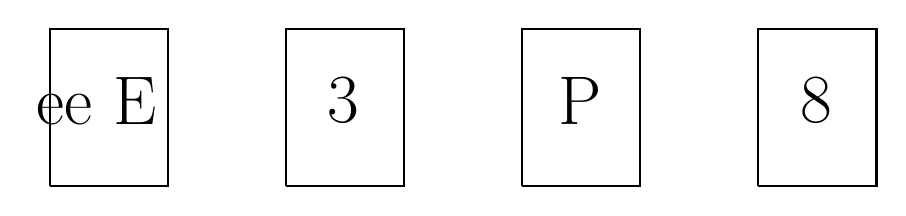
\begin{tikzpicture}
\draw [thick] (0,0)--(0,2)--(1.5,2)--(1.5,0)--(0,0);
\draw [thick] (3,0)--(3,2)--(4.5,2)--(4.5,0)--(3,0);
\draw [thick] (6,0)--(6,2)--(7.5,2)--(7.5,0)--(6,0);
\draw [thick] (9,0)--(9,2)--(10.5,2)--(10.5,0)--(9,0);
\node [below] at (0.6,1.5) {\Huge{\hyperlink{ee}{{ E}}
}};
\node [below] at (3.6,1.5) {\Huge{ 3}};
\node [below] at (6.6,1.5) {\Huge{ P}};
\node [below] at (9.6,1.5) {\Huge{ 8}};
\end{tikzpicture}
\end{center}

Each card has a letter on one side and a number on the other, and I tell you:

\medskip
\begin{block}{}
		 \emph{``\textbf{If} a card has a vowel on one side, \\ 
		 \textbf{then} it has an odd number on the other side." }
\end{block}

	
\medskip
Which cards do you need to turn over in order to verify whether I am telling the truth or not?

%
%
%%%\Large
%
%Four cards lie on the table in front of you.  You know that each card has a letter on one side and a number on the other.  At the moment, you can read the symbols $E$, $P$, $3$, and $8$ on the sides that are up.  I tell you:
%
%\vfill
%
%\begin{block}{}
%		 \emph{``\textbf{If} a card has a vowel on one side, \\ 
%		 \textbf{then} it has an odd number on the other side." }
%\end{block}
%
%\vfill
%
%Which cards do you need to turn over in order to verify whether I am telling the truth or not?
\end{frame}

%------------------------------

\begin{frame}
\frametitle{Cards - 2}

Four cards lie on the table in front of you.  You know that each card has a letter on one side and a number on the other.  

\

{\bf Negate} the following statement:
\begin{block}{}
		 \emph{``\textbf{If} a card has a vowel on one side, \\ 
		 \textbf{then} it has an odd number on the other side." }
\end{block}
\end{frame}



%-----------------------------
\begin{frame}
\frametitle{Negation 2}

Write the negation of this statement without using any negative words (``no", ``not", ``none", etc.): 

\

	\begin{quote}
		``\emph{Every page in this book contains at least one word whose first and last letters both come alphabetically before M.}''
	\end{quote}
\end{frame}

%-----------------------------

\begin{frame}
\frametitle{Negation 3}

Negate the following statement without using any negative words (``no", ``not", ``none", etc.): 

\

	\begin{quote}
		``\emph{I have a friend all of whose former boyfriends had at least two siblings 
	    with exactly three different vowels in their name.}''
	\end{quote}
\end{frame}



\begin{frame}
\frametitle{MAT137 Lecture 5 --- Definitions}
	{\bf Warmup:}

	The law says ``{\bf if you check out a library book, you must return it}''.
	\begin{itemize}
		\item I did not check out any library books.
		\item I did not return any library books.
	\end{itemize}
	Did I violate the law?

	\vfill
	{\bf Before next class:}
		\begin{itemize} \normalsize
			\item {\bf Watch videos 1.14, 1.15 }
		\end{itemize}
	\vfill

\end{frame}

%----------------------------
\begin{frame}
\frametitle{Elephants}

True or False?

\

\begin{enumerate}
	\item  There is a pink elephant in this room.

\

	\item  All elephants in this room are pink.
\end{enumerate}

\end{frame}


%------------------------------

\begin{frame}
\frametitle{One-to-one functions}

Let $f$ be a function with domain $D$.  \\

\vfill

$f$ is \emph{one-to-one} means that ...
	\begin{itemize}
		\item ... different inputs ($\rojo{x}$)  ...
		\item ... must produce different outputs ($\rojo{f(x)}$). 
	\end{itemize}

\vfill
	
\begin{block}{}
	Write a formal definition of ``one-to-one".
\end{block}

\end{frame}


%-----------------------------
\begin{frame}
\frametitle{One-to-one functions}

{\bf Definition:}  Let $f$ be a function with domain $D$.  \\
$f$ is one-to-one means ...
	\begin{enumerate}
		\item  \DS{f(x_1) \neq f(x_2)}
		\item  \DS{\exists x_1, x_2 \in D, \; f(x_1) \neq f(x_2)}
		\item  \DS{\forall x_1, x_2 \in D, \; f(x_1) \neq f(x_2)}
		\item  \DS{\forall x_1, x_2 \in D, \; x_1 \neq x_2, \; f(x_1) \neq f(x_2)}
		\item  \DS{\forall x_1, x_2 \in D, \; x_1 \neq x_2 \implies  f(x_1) \neq f(x_2)}
		\item  \DS{\forall x_1, x_2 \in D, \; f(x_1) \neq f(x_2) \implies  x_1 \neq x_2}
		\item  \DS{\forall x_1, x_2 \in D, \; f(x_1) = f(x_2) \implies x_1 = x_2}
	\end{enumerate}

\end{frame}

%-----------------------------
\begin{frame}
\frametitle{One-to-one functions}

Let $f$ be a function with domain $D$.  \\
{\bf What does each of the following mean?}
	\begin{enumerate}
		\item  \DS{f(x_1) \neq f(x_2)}
		\item  \DS{\exists x_1, x_2 \in D, \; f(x_1) \neq f(x_2)}
		\item  \DS{\forall x_1, x_2 \in D, \; f(x_1) \neq f(x_2)}
		\item  \DS{\forall x_1, x_2 \in D, \; x_1 \neq x_2, \; f(x_1) \neq f(x_2)}
		\item  \DS{\forall x_1, x_2 \in D, \; x_1 \neq x_2 \implies  f(x_1) \neq f(x_2)}
		\item  \DS{\forall x_1, x_2 \in D, \; f(x_1) \neq f(x_2) \implies  x_1 \neq x_2}
		\item  \DS{\forall x_1, x_2 \in D, \; f(x_1) = f(x_2) \implies x_1 = x_2}
	\end{enumerate}

\end{frame}

%-----------------------------
\begin{frame}
\frametitle{Proving a function is one-to-one}
\smallerfont

\begin{block}{Definition}
Let $f$ be a function with domain $D$. \\
We say $f$ is one-to-one when 
	\begin{itemize}
		\item   \hfill \DS{\forall x_1, x_2 \in D, \; x_1 \neq x_2 \implies  f(x_1) \neq f(x_2)}
		\item    OR, equivalently, \hfill  \DS{\forall x_1, x_2 \in D, \; f(x_1) = f(x_2) \implies x_1 = x_2}
	\end{itemize}
\end{block}

\vfill  \p

Suppose I give you a specific function $f$ and I ask you to prove it is one-to-one.  \pause
	\begin{itemize} 
		\item {\bf For the first definition}, write the structure of your proof (How do you begin? What do you assume? What do you conclude?).
		\item {\bf For the second definition}, write the structure of your proof if you use the second definition.
	\end{itemize}
	
\vfill	  \p

\begin{block}{Exercise}
	Prove that $f(x) = 3x + 2$, with domain $\R$, is one-to-one.
\end{block}

\end{frame}



\begin{frame}
	\frametitle{MAT137 Lecture 6 --- Proofs \& Induction}

	{\bf Warmup:}

	For each of the following statements, list {\bf all} conditions under which it is false.
	\begin{itemize}
		\item If a student gets a 100 on the test, I will give them a cookie.
		\item If I check out a library book, I will return it.
		\item If there is an elephant in this room, it is pink.
	\end{itemize}
	\vfill
	{\bf Before next class:}
		\begin{itemize} \normalsize
			\item {\bf Watch videos 2.4 }
		\end{itemize}
	\vfill

\end{frame}

\begin{frame}
\frametitle{Cookies Redux}
	A teacher promises: \textbf{If a student gets a 100 on the test, then I will give them a cookie.}
	\begin{itemize}
		\bigskip
		\item No student gets 100.
		\item The teacher doesn't give out any cookies.
	\end{itemize}
		\vfill
	Did the teacher lie?

\vfill

\end{frame}

\begin{frame}
\frametitle{Library Redux}
	The law says, ``{\bf If you check out a library book, you must return it}''.
	\bigskip
	\begin{itemize}
		\item I did not check out any library books.
		\item I did not return any library books.
	\end{itemize}

	\vfill
	Did I violate the law?
\vfill
\end{frame}

\begin{frame}
\frametitle{Elephant Redux}
	Consider the statement ``{\bf if this room contains an elephant, that elephant is pink}''.

	\bigskip
	The facts are:
	\begin{itemize}
		\item This room contains no elephants.
		\item If there were an elephant in this room, it would come from the zoo and would be a grey elephant.
	\end{itemize}
	\vfill
	Is the statement true or false?
\vfill
\end{frame}

\begin{frame}
\frametitle{My Mind}
	Consider the statements
	\bigskip
	\begin{enumerate}
		\item If I have a favorite number, then it is an even number.
		\item If I have a favorite number, then it is an odd number.
	\end{enumerate}

	\vfill
	Can both statements be true at the same time?
\vfill
\end{frame}


%-----------------------------
\begin{frame}[t]
\fontsize{13}{13}\selectfont
\frametitle{Proving a function is NOT one-to-one}

\begin{block}{Definition}
Let $f$ be a function with domain $D$. \\
We say $f$ is one-to-one when 
	\begin{itemize} 
		\item   \hfill \DS{\forall x_1, x_2 \in D, \; x_1 \neq x_2 \implies  f(x_1) \neq f(x_2)}
		\item    OR, equivalently, \hfill  \DS{\forall x_1, x_2 \in D, \; f(x_1) = f(x_2) \implies x_1 = x_2}
	\end{itemize}
\end{block}

\vfill  \p

	Suppose I give you a specific function $f$ and I ask you to prove it is \textbf{not} one-to-one. \pause  You need to prove $f$ satisfies the \emph{negation} of the definition.
	\begin{itemize}
		\item  Write the negation of the first definition.
		\item  Write the negation of the second definition.
		\item  Write the structure of your proof. 
	\end{itemize}
	
\vfill	 \p

\begin{block}{Exercise}
	Prove that $f(x) =  x^2$, with domain $\R$, is not one-to-one.
\end{block}

\end{frame}



%------------------------------
\begin{frame}
\frametitle{Variations on induction}

Let $S_n$ be a statement depending on a positive integer $n$.

\vfill  

	What conclusions can you draw in each of the following cases? (I.e., for which $n$ do you
	know that $S_n$ is true?)

\vfill 

\begin{multicols}{2}
\begin{enumerate}
\item  We have proven:
	\begin{itemize}
		\item   $S_3$ 
		\item  \DS{\forall n \geq 1, \; S_{n}  \implies S_{n+1} }
	\end{itemize}	
\item  We have proven:
	\begin{itemize}
		\item  $S_1$ 
		\item  \DS{\forall n \geq 3, \; S_{n} \implies S_{n+1} }
	\end{itemize}	
\item  We have proven:
	\begin{itemize}
		\item  $S_1$ 
		\item  \DS{\forall n \geq 1, \; S_{n} \implies S_{n+3} }
	\end{itemize}	
\item  We have proven:
	\begin{itemize}
		\item  $S_1$ 
		\item  \DS{\forall n \geq 1, \; S_{n+1}  \implies S_{n} }
	\end{itemize}	
\end{enumerate}	
\end{multicols}

\vfill

\end{frame}


%-----------------------------
\begin{frame}
\frametitle{Variations on induction 2}

We want to prove  
	$$\forall n \geq 1, \; S_n $$
	
\vfill

So far we have proven
	\begin{itemize}
		\item  $S_1$ 
		\item  \DS{\forall n \geq 1, \; S_n \implies S_{n+3}.}
	\end{itemize}	

\vfill	

What else do we need to do?

\end{frame}

%----------------------------
\begin{frame}
\frametitle{What is wrong with this proof by induction?}
\smallerfont

\vspace{-1.5mm}
\begin{theorem}
$\forall N \geq 1$, every set of $N$ students in MAT137 will get the same grade.
\end{theorem} \p
\vspace{-1mm}

\begin{proof}
\begin{itemize} 
	\item  {\bf Base case.}  It is clearly true for $N=1$.
	\item  {\bf Induction step.}  \\
		Assume it is true for $N$.  I'll show it is true for $N+1$. \\
		Take a set of $N+1$ students.  By induction hypothesis:
			\begin{itemize}
				\item  The first $N$ students get the same grade.
				\item  The last $N$ students get the same grade.
			\end{itemize}
			$$
				\mathrlap{\overbrace{\phantom{\bullet \quad \bullet \quad \cdots \quad \bullet \quad \bullet }}^{\text{Same grade}}}
				\bullet \quad \underbrace{\bullet \quad \bullet \quad \cdots \quad \bullet \quad \bullet}_{\text{Same grade}}
			$$
		Hence the $N+1$ students all get the same grade.
\end{itemize}
\end{proof}

\end{frame}
%----------------------------
\begin{frame}
\frametitle{What is wrong with this proof by induction?}

For every $N \geq 1$, let
	\begin{center}
	\begin{tabular}{rcc}
		\DS{S_N} =  & ``every set of $N$ students in MAT137 \\ & will get the same grade"
	\end{tabular}
	\end{center}

\vfill 

What did we actually prove in the previous page?

	\begin{itemize}
		\item  $S_1$ \, ?
		\item  \DS{\forall N \geq 1}, \, \DS{S_N \implies S_{N+1}} \, ?
	\end{itemize}

\vfill 
\end{frame}

%-----------------------------
\begin{frame}
\frametitle{What is wrong with this proof? (1)}

\begin{block}{Theorem}
The sum of two odd numbers is even.
\end{block}
 
	\vfill

\begin{proof}
3 is odd.  \\
5 is odd. \\
$3+5 = 8$ is even.
\end{proof}

\vfill

\end{frame}
%-----------------------------
\begin{frame}
\frametitle{What is wrong with this proof? (2)}


\begin{block}{Theorem}
The sum of two odd numbers is even.
\end{block}

 \vfill

\begin{proof}
The sum of two odd numbers is always even.  \\
even + even = even \\
even + odd = odd \\
odd + even = odd \\
odd + odd = even.
\end{proof}

\vfill

\end{frame}
%-----------------------------
%\begin{frame}
%\frametitle{Symmetric difference}
%
%Given two sets $A$ and $B$, we define
%\begin{itemize}
%	\item  $A \setminus B = \{  x \in A \; : \; x \notin B \}$
%	\item $A \triangle B = (A \setminus B) \cup (B \setminus A)$
%\end{itemize}
%
%\vfill
%
%Let
%\begin{itemize}
%	\item  $C_1 = \{ \mbox{  students under 18 } \}$
%	\item  $C_2 = \{ \mbox{ students born in Ontario } \}$
%\end{itemize}
%
%\vfill
%
%What is the set $C_1 \triangle C_2$?
%
%\vfill
%
%\end{frame}
%%-----------------------------
%\begin{frame}
%\frametitle{Symmetric difference - 2}
%
%Given two sets $A$ and $B$, we define
%\begin{itemize}
%	\item  $A \setminus B = \{  x \in A \; : \; x \notin B \}$
%	\item $A \triangle B = (A \setminus B) \cup (B \setminus A)$
%\end{itemize}
%
%\vfill
%
%Is the following equality
%$$
%	(A \triangle B) \triangle C \; = \; A \triangle (B \triangle C)
%$$
%true for all sets $A$, $B$, and $C$?
%
%\vfill
%
%\end{frame}
%------------------------------

%\begin{frame}[t]
%\frametitle{Even numbers}
%
%Write a description of the set $E$ of even integers using set-building notation.
%
%\end{frame}
%
%
%%-----------------------------
%\begin{frame}
%\frametitle{Indecisive function}
%
%Construct a function $f$ that satisfies all of the following properties at once:
%	\begin{itemize}
%		\item  The domain of $f$ is $\R$.
%		\item  \DS{\forall x \in \R, \exists y \in \R} such that
%			$$  x<y \mbox{ and } f(x) < f(y) $$
%		\item  \DS{\forall x \in \R, \exists y \in \R} such that
%			$$  x<y \mbox{ and } f(x) > f(y) $$
%	\end{itemize}
%
%\end{frame}
%%-----------------------------
%
%\begin{frame}
%\frametitle{Graphs}
%
%Draw the graph of a function $f$ with domain $\mathbb{R}$ that satisfies:
%	\begin{equation*}
%		\mbox{If } 2<x<4 \mbox{ then } 1<f(x)<2.  	
%	\end{equation*}
%\vfill
%
%Draw the graph of a function $g$ with domain $\mathbb{R}$ that satisfies:
%	\begin{equation*}
%		2<x<4 \mbox{ if and only if } 1 < g(x) < 2.
%	\end{equation*}
%\vfill
%
%\end{frame}
%
%
%%-----------------------------
%
%\begin{frame}
%\frametitle{Proving a theorem}
%
%\begin{block}{Theorem}
%	Let $f$ be a function with domain $D$.
%		\begin{itemize}
%			\item  IF $f$ is increasing on \DS{D}
%			\item  THEN $f$ is one-to-one on \DS{D}
%		\end{itemize}
%\end{block}
%
%\vfill  \p
%
%\begin{enumerate}
%	\item  Remind yourself of the precise definition of ``increasing" and ``one-to-one". \p
%	\item  To prove the theorem, what will you assume?  what do you want to show? \p
%	\item   Look at the part you want to show.  Based on the definition, what is the structure of the proof? \p
%	\item   Complete the proof. 
%\end{enumerate}
%
%\end{frame}
%
%%-----------------------------
%
%\begin{frame}
%\frametitle{DISproving a theorem}
%
%\begin{block}{ FALSE Theorem}
%	Let $f$ be a function with domain $D$.
%		\begin{itemize}
%			\item  IF $f$ is one-to-one on \DS{D}
%			\item  THEN $f$ is increasing on \DS{D}
%		\end{itemize}
%\end{block}
%
%\vfill  \p
%
%\begin{enumerate}
%	\item  This theorem is false.  What do you need to do to prove it is false? \p
%	\item  Prove the theorem is false.
%\end{enumerate}
%
%\end{frame}
%
%%-----------------------------
%\begin{frame}
%\frametitle{Definition of odd and even}
%
%Write a definition of ``odd integer" and ``even integer".
%
%\p \vfill
%
%\begin{block}{Definition}
%  Let $x \in \Z$.  We say that $x$ is odd when ...
%	\begin{enumerate}
%		\item  $x = 2a+1$ ?
%		\item  \DS{\forall a \in \Z, x = 2a+ 1 }?
%		\item  \DS{\exists a \in \Z \mbox{ s.t. } x = 2a+ 1 }?
%	\end{enumerate}
%\end{block}
%
%	
%\vfill
%	
%\end{frame}
%
%%-----------------------------
%\begin{frame}
%\frametitle{What is wrong with this proof? (3)}
%
%\begin{block}{Theorem}
%The sum of two odd numbers is always even.
%\end{block}
%
%
%\pause
%
%\begin{proof}
%\DS{x= 2a + 1} odd 
%
%\DS{y = 2b + 1} odd 
%
%\DS{ x+ y = 2n}  even 
%
%\DS{2a + 1 + 2b + 1 = 2n} 
%
%\DS{2a + 2b + 2 = 2n}
%
%\DS{a + b + 1 = n}
%\end{proof}
%\end{frame}
%
%%-----------------------------
%
%
%\begin{frame}
%\frametitle{Write a correct proof!}
%
%\begin{block}{Theorem}
%The sum of two odd numbers is always even.
%\end{block}
%
%\end{frame}
%
%
%
%%-----------------------------
%\begin{frame}
%\frametitle{Variations on induction 3}
%
%We want to prove  
%	$$\forall n \in \Z, \; S_n $$
%	
%\vfill
%
%So far we have proven
%	\begin{itemize}
%		\item  $S_1$
%	\end{itemize}	
%
%\vfill	
%
%What else do we need to do?
%
%\end{frame}


%------------------------------
%------------------------------
%-----------------------------
\end{document}
%-----------------------------
%-----------------------------
%-----------------------------









